\begin{appendices}


\section{TL plots for experiments in \cref{sec:pretrain-freeze}}
\label{sec:pretrain-freeze-TL}

\begin{figure}[ht]
    \centering
    \begin{subfigure}[t]{0.4\textwidth}
       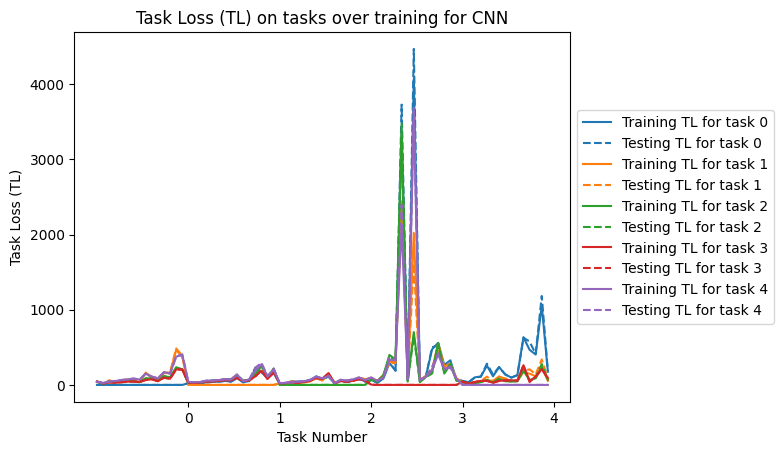
\includegraphics[width=\linewidth]{images/CIFAR10_CL/CNN_TL_task.png}
       \caption{TL's over training for the CNN on split-CIFAR10. We see that over the course of each task the loss obtained on tasks increases and that the loss of the current task being trained on decreases, we also see a big spike in the loss during training on task 2.}
    \end{subfigure}
    \quad % add space between images
    \begin{subfigure}[t]{0.4\textwidth}
       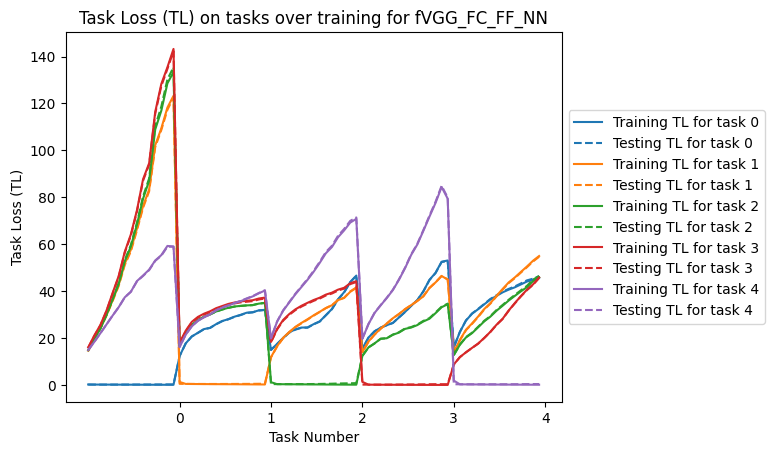
\includegraphics[width=\linewidth]{images/CIFAR10_CL/fVGG_FC_FF_NN_TL_task.png}
       \caption{TL's over training for the fVGG-FCFFNN on split-CIFAR10. We see that over the course of each task the loss obtained on tasks increases and that the loss of the current task being trained on decreases.}
    \end{subfigure}
    
    \medskip % add space between rows
    
    \begin{subfigure}[t]{0.4\textwidth}
       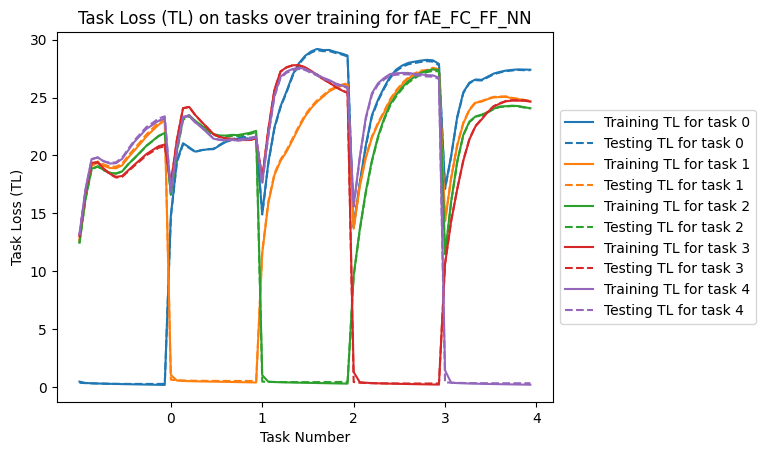
\includegraphics[width=\linewidth]{images/CIFAR10_CL/fAE_FC_FF_NN_TL_task.png}
       \caption{TL's over training for the fAE-FCFFNN on split-CIFAR10. We see that over the course of each task the loss obtained on tasks increases and that the loss of the current task being trained on decreases.}
    \end{subfigure}
    \quad % add space between images
    \begin{subfigure}[t]{0.4\textwidth}
       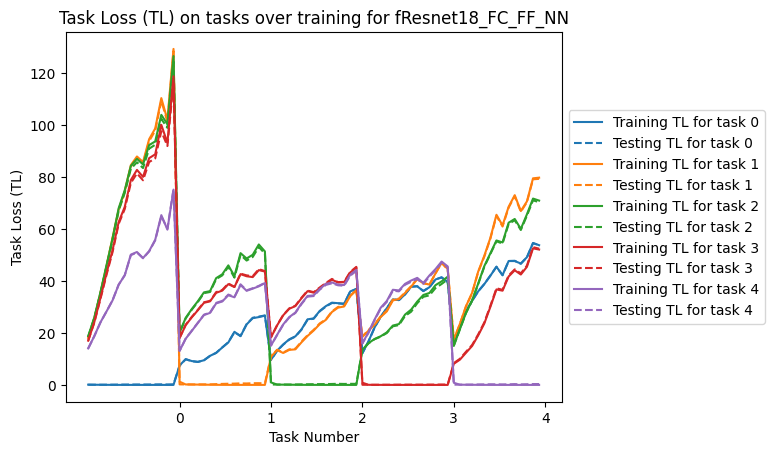
\includegraphics[width=\linewidth]{images/CIFAR10_CL/fResnet18_FC_FF_NN_TL_task.png}
       \caption{TL's over training for the fResnet18-FCFFNN on split-CIFAR10. We see that over the course of each task the loss obtained on tasks increases and that the loss of the current task being trained on decreases.}
    \end{subfigure}

    \medskip % add space between rows

    \begin{subfigure}[t]{0.4\textwidth}
      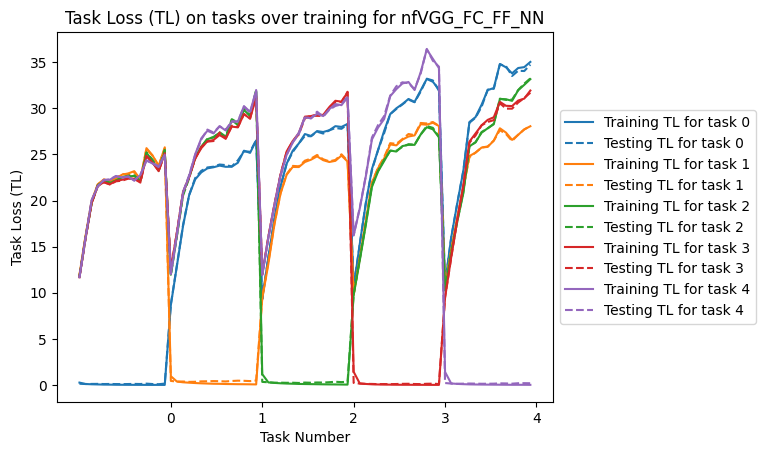
\includegraphics[width=\linewidth]{images/CIFAR10_CL/nfVGG_FC_FF_NN_TL_task.png}
      \caption{TL's over training for the nfVGG-FCFFNN on split-CIFAR10. We see that over the course of each task the loss obtained on tasks increases and that the loss of the current task being trained on decreases.}
   \end{subfigure}
   \quad % add space between images
   \begin{subfigure}[t]{0.4\textwidth}
      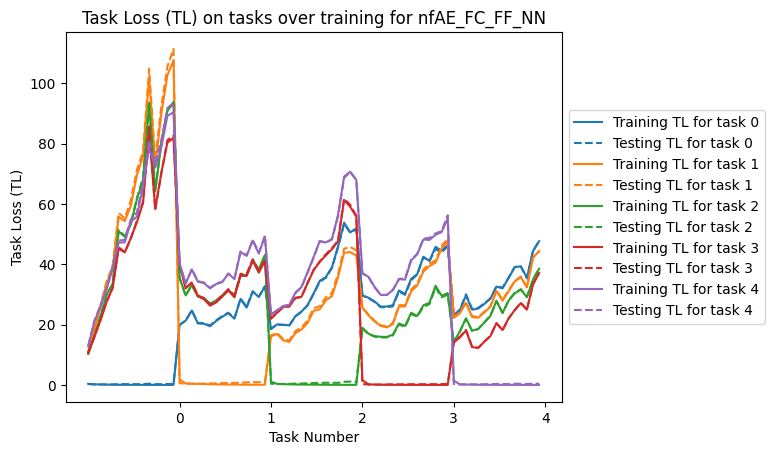
\includegraphics[width=\linewidth]{images/CIFAR10_CL/nfAE_FC_FF_NN_TL_task.png}
      \caption{TL's over training for the nfAE-FCFFNN on split-CIFAR10. We see that over the course of each task the loss obtained on tasks increases and that the loss of the current task being trained on decreases.}
   \end{subfigure}

    \medskip % add space between rows

    \begin{subfigure}[t]{0.4\textwidth}
      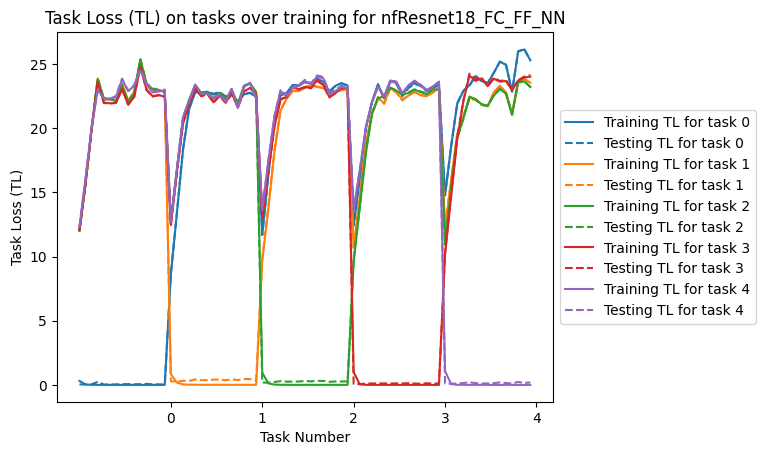
\includegraphics[width=\linewidth]{images/CIFAR10_CL/nfResnet18_FC_FF_NN_TL_task.png}
      \caption{TL's over training for the nfResnet18-FCFFNN on split-CIFAR10. We see that over the course of each task the loss obtained on tasks increases and that the loss of the current task being trained on decreases.}
   \end{subfigure}
    
    \caption{The testing and training TL's on each individual task over training epochs for all the networks we trained on split-CIFAR10.}
    \label{fig:CIFAR10-CL-TL}
\end{figure}

\FloatBarrier
\section{Compute times and TL plots for experiments in \cref{sec:resetting}}
\label{sec:resetting-TL}

\begin{figure}[ht]
    \centering
    \begin{subfigure}[t]{0.4\textwidth}
       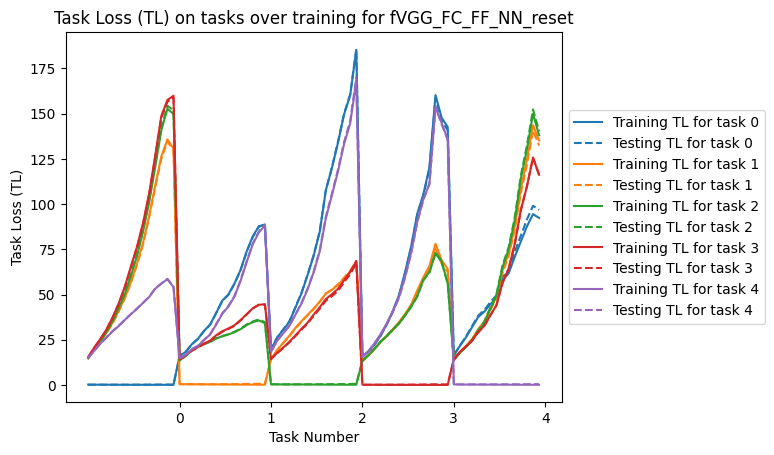
\includegraphics[width=\linewidth]{images/CIFAR10_CL/fVGG_FC_FF_NN_reset_TL_task.png}
       \caption{All the TL's for the fVGG-FCFFNN with reset over training, it's results mirror extremely closely the results of the fVGG-FCFFNN without reset.}
    \end{subfigure}
    \quad
    \begin{subfigure}[t]{0.4\textwidth}
       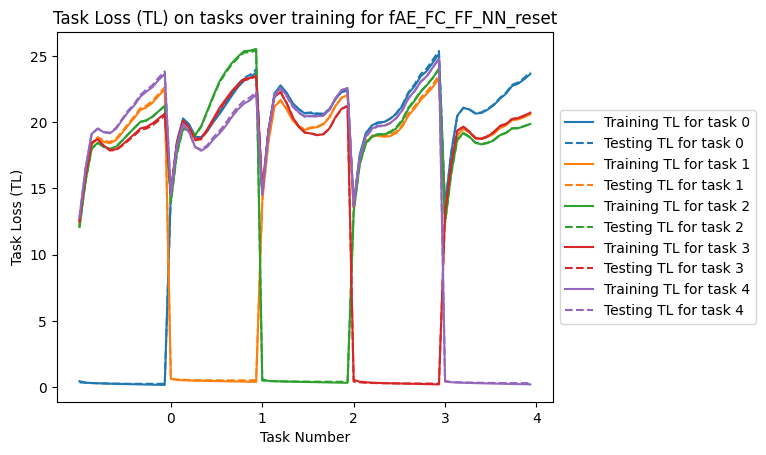
\includegraphics[width=\linewidth]{images/CIFAR10_CL/fAE_FC_FF_NN_reset_TL_task.png}
       \caption{All the TL's for the fAE-FCFFNN with reset over training, it's results mirror extremely closely the results of this network without reset.}
    \end{subfigure}
    
    \medskip % add space between rows
  
    \begin{subfigure}[t]{0.4\textwidth}
       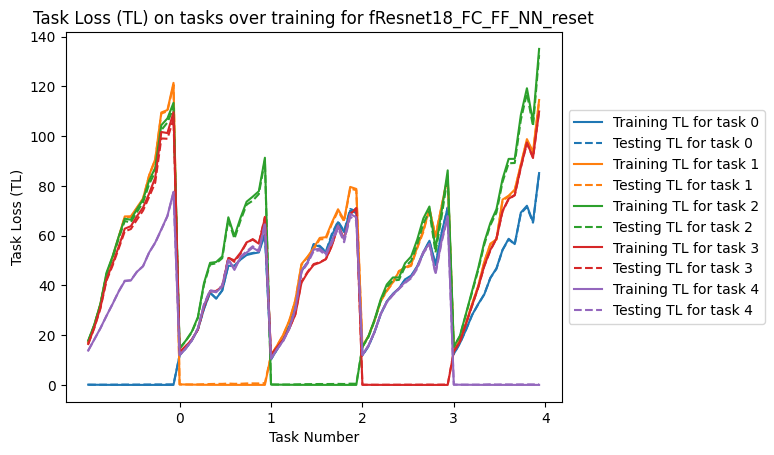
\includegraphics[width=\linewidth]{images/CIFAR10_CL/fResnet18_FC_FF_NN_reset_TL_task.png}
       \caption{All the TL's for fResnet18-FCFFNN with reset over training, it achieves very similar results to the fResnet18-FCFFNN without reset. Except with reset the more gradual forgetting isn't witnessed (as would be expected randomly initializing the head of the network).}
    \end{subfigure}
    \quad
    \begin{subfigure}[t]{0.4\textwidth}
      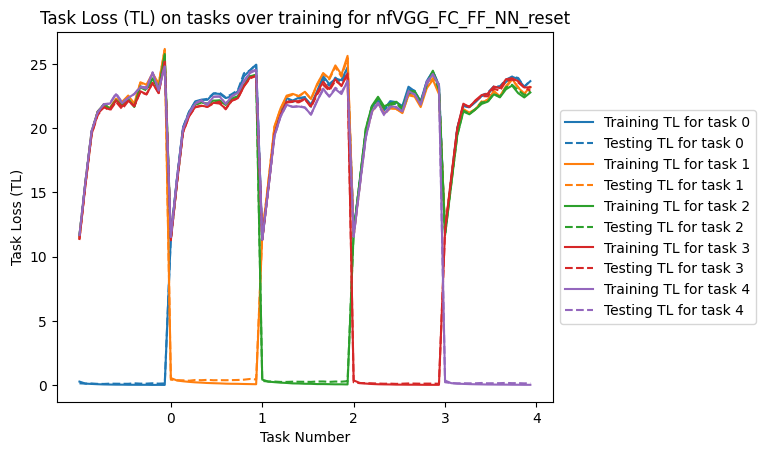
\includegraphics[width=\linewidth]{images/CIFAR10_CL/nfVGG_FC_FF_NN_reset_TL_task.png}
      \caption{All the TL's for nfVGG-FCFFNN with reset over training, it's results closely resemble the results of this network without reset.}
   \end{subfigure}
   
   \medskip % add space between rows
  
   \begin{subfigure}[t]{0.4\textwidth}
      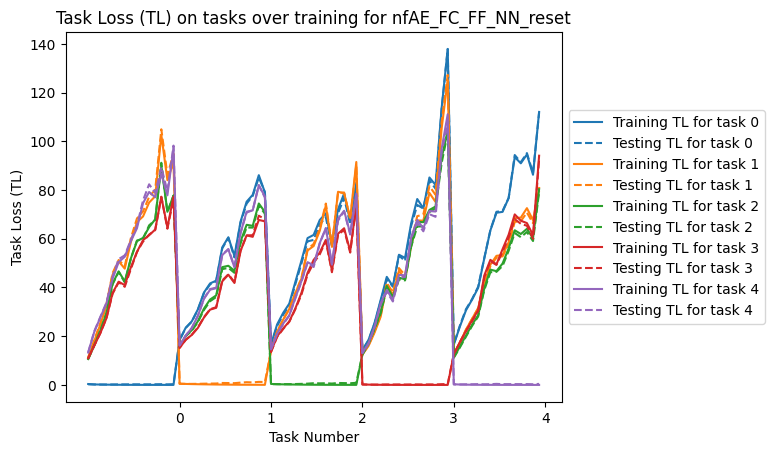
\includegraphics[width=\linewidth]{images/CIFAR10_CL/nfAE_FC_FF_NN_reset_TL_task.png}
      \caption{All the TL's for nfAE-FCFFNN with reset over training, it's results also closely resemble the results without reset, except for a slightly more gradual learning curve when it's just started training on a new task.}
   \end{subfigure}
   \quad
    \begin{subfigure}[t]{0.4\textwidth}
      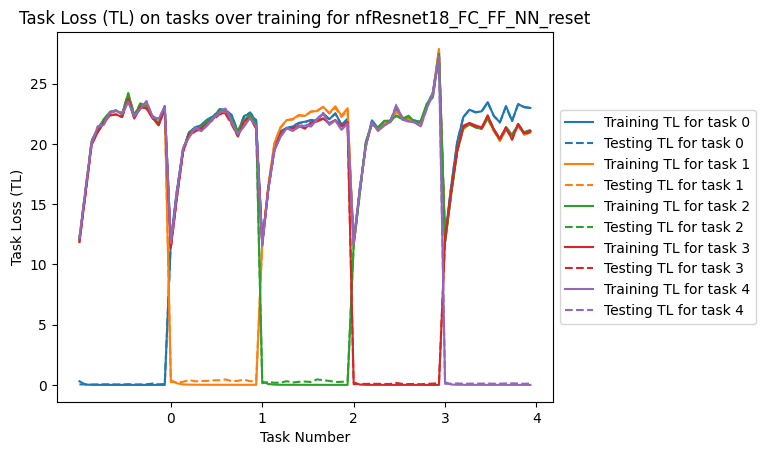
\includegraphics[width=\linewidth]{images/CIFAR10_CL/nfResnet18_FC_FF_NN_reset_TL_task.png}
      \caption{All the TL's for nfResnet18-FCFFNN with reset over training, it's results also closely resemble the results of this network without reset.}
   \end{subfigure}
    
    \caption{The testing and training TL's on each individual task over training epochs for all the networks we trained on split-CIFAR10.}
    \label{fig:CIFAR10-CL-TL-reset}
\end{figure}

\begin{table}[ht]
    \centering
    \begin{tabular}{l c}
    \toprule
    \textbf{Model Name} & \textbf{Total compute time (seconds)} \\
    \midrule
    \textbf{fVGG-FCFFNN-reset} & 5559.18 \\
    \textbf{nfVGG-FCFFNN-reset} &  22605.64 \\
    \textbf{fAE-FCFFNN-reset} &  6435.23 \\
    \textbf{nfAE-FCFFNN-reset} &  7740.14 \\
    \textbf{fResnet18-FCFFNN-reset} & \textbf{5425.43}  \\
    \textbf{nfResnet18-FCFFNN-reset} &  31206.32 \\
    \bottomrule
    \end{tabular}
    \caption{Table of compute times and total number of trainable parameters of our models trained on split-CIFAR10 with reset, one NVIDIA GeForce RTX 2080 Ti was used to train each of these models.}
    \label{tab:compute_times_reset}
\end{table}

\FloatBarrier
\section{Hyperparameters used for all experiments}
\label{sec:hyperparameters}
The networks as described in \cref{subsec:networks} is how we kept them for all experiments, the only things that changed was in split-CIFAR10 we reset the Adam optimizer at the beginning of each task and we used different learning rates. We will now run through the learning rates we used for each experiment. With MNIST we used the same learning rates in the CL and batch scenarios and trained in both scenarios using SGD:
\begin{itemize}
    \item \textbf{FCFFNN} - 0.007
    \item \textbf{CNN} - 0.005
\end{itemize}
With CIFAR10 we used the Adam optimizer with the following learning rates:
\begin{itemize}
    \item \textbf{CNN} - 0.0001
    \item \textbf{nfVGG-FCFFNN} - 0.0008
    \item \textbf{fVGG-FCFFNN} - 0.0008
    \item \textbf{nfResnet18-FCFFNN} - 0.002
    \item \textbf{fResnet18-FCFFNN} - 0.002
    \item \textbf{nfAE-FCFFNN} - 0.001
    \item \textbf{fAE-FCFFNN} - 0.0025
\end{itemize}
With split-CIFAR10 we used the Adam optimizer and reset it at the beginning of each task with the following learning rates:
\begin{itemize}
    \item \textbf{CNN} - 0.0001
    \item \textbf{nfVGG-FCFFNN} - 0.00001
    \item \textbf{fVGG-FCFFNN} - 0.00005
    \item \textbf{nfResnet18-FCFFNN} - 0.00001
    \item \textbf{fResnet18-FCFFNN} - 0.00005
    \item \textbf{nfAE-FCFFNN} - 0.00005
    \item \textbf{fAE-FCFFNN} - 0.00005
\end{itemize}
We used the same learning rates above in the reset experiments.

\end{appendices}